\hypertarget{sec:requirements-analysis}{%
\chapter{Requirements Analysis}\label{sec:requirements-analysis}}

In this chapter, we further investigate the problem raised in the introduction -- concerns about effort and risk that render \glspl{isv} hesitant to commence a \gls{Web Migration} due to insufficient support in initial phases -- by outlining the research context in an industrial scenario, analyzing the specific problems within the scenario and through the derivation of concrete requirements.

\vspace{-15pt}
\hypertarget{sec:scenario}{%
\section{Scenario}\label{sec:scenario}}
\vspace{15pt}

The following scenario describes the external industrial context in which the research presented in this thesis was conducted.
It provides a concrete real-world example of the problems described in \cref{sec:problem}.
The scenario's characteristics with regard to company, software development, and \gls{source system} provide the basis for the detailed problem analysis in \cref{sec:problem-analysis} and provide contextual information for the solution elaborated in \cref{sec:solution}.

\vspace{-10pt}
\hypertarget{sec:company-characteristics}{%
\subsection[Company \& Software Development Characteristics]{Company and Software Development Characteristics}\label{sec:company-characteristics}}
\vspace{10pt}

The scenario is based on the situation of \emph{medatixx GmbH \& Co.~KG} at the beginning of the joint industrial research project ``eHealth Research Laboratory'' in October 2014.
Medatixx is a \gls{sme}-sized \gls{isv} of about 130 software developers plus 360 additional service and sales employees \autocite{Medatixx2018}.
Like most \gls{sme} \glspl{isv} \autocite{Rose2016InnovationSME}, medatixx is successfully specialized in one particular sector, providing software solutions and IT Services for all kinds of resident doctors' offices and is the largest software provider in this sector in Germany with a market share of about 22\% \autocite{Medatixx2018}.
The core software development activities focus on information systems for patient management, so-called \glspl{pms}.
This type of software is subject to various regulatory constraints: general rulings like the GDPR to ensure data privacy \autocite{GDPR2016} as well as regulations specific to the medical sector like required certifications of \gls{pms} through the federal association of statutory health insurance physicians (KBV) \autocite{KBV2018}.
Updated regulations also impose a strict regime of quarterly release cycles that influences developer workload, maintenance activities, and evolution practices of the software products.
It is worth noting that the business processes in many doctors' offices are based on the processes represented in the \gls{pms}, making it hard to introduce more substantial changes in user interaction patterns or even replace the \gls{pms}.
As a result of several mergers and existing contracts with customers for maintenance and updates, the company continuously develops and evolves four similar main software products with overlapping features, different technologies, and partially shared codebases.
Modernization activities are viewed in an in-house context; outsourcing is not desired.
The development staff is experienced in the technology bases and the functionality of the existing software products, but due to time and the mergers, the original developers and expertise are not entirely available anymore.
\gls{Web Engineering} expertise is only limited; \gls{Web Migration} expertise was not observed.
Incremental \glslink{Software Modernization}{modernization} of older software components is ongoing, focussing on re-development in C\#.NET.
%A previous migration attempt towards a client/server architecture failed due to the complexity and lack of sufficient resources.

The software development activities are organized following agile practices and adoption of agile culture and mindset in work, and decision processes are at an advanced level for both software developers and the management of the development department.
The software developers are organized in teams of about 5-7 persons and integrate domain experts as testers.
These teams complete work from backlogs managed by product managers in a self-organized way.
Except for one team dedicated to corrective maintenance, which adopts a Kanban \autocite{Anderson2010Kanban} process, the teams follow a Scrum-based \autocite{Beedle2002Scrum} iterative development model with minor variations across different teams.
Implementations of new features need to be approved by a group of \gls{uix} experts (Team U) to ensure consistently high usability.
Further agile methods and technologies such as physical sprint backlogs, time-framed efficient meetings with voluntary participation, continuous integration, and automated software testing as well as knowledge sharing approaches like a gamification-driven wiki are present.
The above description characterizes medatixx as a typical instance of the \emph{main stakeholder role} of this thesis: a capable modern \gls{sme}-sized \gls{isv} with the problem of bringing its non-\glslink{web}{Web} \glspl{Legacy System} to the \gls{web}.

\vspace{-10pt}
\hypertarget{sec:scenario-code}{%
\subsection{Legacy Codebase Characteristics}\label{sec:scenario-code}}
\vspace{10pt}

For our joint research, we were kindly given access to the source code of one of the \gls{pms} called \emph{x.concept} by medatixx.
It provides functionality encompassing patient documentation and health records, managing appointments, prescriptions, and billing, focused on \gls{crud} operations.
The application is a traditional \emph{stand-alone \gls{Desktop Application} with a \gls{gui}}, distributed via optical media and deployed via local installation on Windows-based personal computers in doctors' offices.
For distributed access from several workstations in different rooms, some doctors' offices are using MS Remote Desktop connections to a central PC that plays a server-like role.
To provide an overview of the general characteristics of the codebase, we used the source code analysis tool \emph{cloc}\footnote{\url{https://github.com/AlDanial/cloc} Retrieved: 6.12.2019} version 1.80.
The source code consists of 34269 files, 30840 of which are unique (redundancy is mainly due to duplicate C/\cpp Header files and some amount of code duplication), with an aggregated number of 8.8 million \gls{sloc}.
Source code analysis identified a heterogeneous landscape of 28 different programming languages and technologies, the vast majority of which (16.6k files, 6.5M \gls{sloc}) is Visual \cpp.
Other programming languages include C\# (7.2k files, 1.5M \gls{sloc}), C (244 files, 163k \gls{sloc}), and Pascal (150 files, 100k \gls{sloc}), technology-related \glspl{artifact} include \gls{html} (588 files, 149k \gls{sloc}), Windows Resource Files (767 files, 107k \gls{sloc}), MSBuild Scripts (437 files, 55k \gls{sloc}) and \gls{xaml}\footnote{\url{http://msdn.microsoft.com/en-us/library/ms747122.aspx} Retrieved: 6.12.2019} (122 files, 17.8k \gls{sloc}).
The main technologies are Visual \cpp as programming language, \gls{mfc}\footnote{\url{http://msdn.microsoft.com/de-de/library/d06h2x6e.aspx} Retrieved: 6.12.2019} as \gls{gui} framework and FoxPro for persistence.
Further details can be found in \cref{tbl:zms-analysis}.
The software is structured in mostly isolated components, in some cases even stand-alone ones with several different communication mechanisms such as COM, IPC/Sockets, and \gls{mfc} SendMessage.
While advanced metrics like functional size measurement (FSM) \autocite{ISO/IEC2009FSM} would provide more insight into the amount of functionality, automated calculation of function points is still not mature, and due to correlation with lines of code metrics \autocite{Albrecht1983FP} their improved objectivity has been questioned.
In any case, the size of 8.8M \gls{sloc} clearly qualifies x.concept as a large\footnote{only 12\% of the applications in the Appmarq repository --- representing 1.03 billion \gls{loc} of 1850 applications --- are larger than 1M \gls{loc} \autocite{CAST2017}} \gls{Legacy System}.

Within x.concept, \emph{ZMS} is an isolated stand-alone component, that compiles into a separate executable handling the management of medical appointments.
It provides standard calendar functionality like day, 3-day, week and month calendar views, a task list, a vacation planner, a business hours schedule, and management of patient appointments involving resources from medical staff and rooms.
Data flows for appointments go directly to an MS SQL Server via ODBC, whereas resource data is loaded through Window-to-Window communication with the main application via \gls{mfc} SendMessage.
ZMS serves as scenario application basis in this thesis.
\Cref{tbl:legacy_characteristics} shows abstract characteristics of the type of \glslink{Legacy System}{legacy} software which we focus on in this thesis along with their instantiation in the ZMS scenario application.

\hypertarget{tbl:legacy_characteristics}{}
\begin{longtable}[]{@{}lp{6cm}@{}}
\caption[Legacy Software Characteristics \& Scenario Instantiation]{\label{tbl:legacy_characteristics}Abstract Technical Characteristics of Legacy Software \& Scenario Instantiation \autocite[adapted from][]{Heil2018ReWaMP}}\tabularnewline
\toprule
Abstract Characteristics & Instantiation in ZMS scenario application\tabularnewline
\midrule
\endfirsthead
\toprule
Abstract Characteristics & Instantiation in ZMS scenario application\tabularnewline
\midrule
\endhead
Legacy language & Visual \cpp\tabularnewline
\gls{crud} functionality & \gls{crud} for medical appointments\tabularnewline
Complex Business Logic & find next available time slot\tabularnewline
Desktop GUI & Microsoft Foundation Class (\gls{mfc})\tabularnewline
Component Communication & Window-to-Window via \gls{mfc} SendMessage\tabularnewline
Third-party dependencies & DLLs via assembly loading\tabularnewline
File and Data Base Persistence & Files and MS SQL Server via ODBC\tabularnewline
\bottomrule
\end{longtable}

%\vspace{-20pt}
%\vspace{-10pt}
\pagebreak
\hypertarget{migration-objectives}{%
\subsection{Migration Objectives}\label{migration-objectives}}
\vspace{10pt}

Current \gls{pms} like x.concept primarily support doctors and nurses.
Future healthcare applications, however, should support all roles involved in ambulant healthcare, such as patients, pharmacists, or transport providers.
The situation is comparable to the banking sector twenty years ago when banking information systems only supported bank clerks as actors.
With the increasing ubiquity of \glslink{web}{Web}-based systems, the extension of these formerly closed systems empowering customers as system actors has lead to the successful establishment of online banking as the de-facto standard for internet users \autocite{BitkomResearch2016DigitalBanking} and enabled the creation of new business models creating the FinTech sector \autocite{Schueffel2016FinTech}.
Similar effects have been observed for the travel sector.
Empowering the physicians' customers, i.e.~the patients, in the context of the ZMS scenario application means the following: to provide them with functionality to book their medical appointments based on availability and personal preferences, to re-schedule or cancel appointments, to receive reminders and delay notifications and to access this information independent of the doctors' business hours and integrate the appointments in calendar applications on the patients' personal mobile devices.
Comparable functionality is familiar for end users, e.g.~in the context of flight bookings.
Providing this increased functionality and comfort to patients -- the customers of the company's customers -- generates an added value and a potential competitive advantage for doctors -- the customers of the company -- and therefore is desirable for the \gls{pms} of the \gls{isv}.

To enable this, however, a distributed, \glslink{web}{Web}-based system is required, using open \gls{web} standards to provide a high degree of interoperability.
The current locally installed, closed \gls{pms} cannot deliver the required interactivity, because its installations run on PCs in the doctors' offices -- often only during business hours -- and cannot be accessed or interacted with from outside.
Integration of further third-party roles like pharmacists and transport providers for federated scenarios would require standardized communication interfaces and authorization mechanisms.
The required \gls{Web Migration} poses a challenge for the \gls{isv}, and initiating this process is difficult as outlined in \cref{sec:problem} and further analyzed in \cref{sec:problem-analysis-results}.

\vspace{-15pt}
\hypertarget{sec:problem-analysis}{%
\section{Problem Analysis}\label{sec:problem-analysis}}
\vspace{15pt}

\emph{Effort and risk} were identified as the two main problems in \cref{sec:introduction}.
This section analyzes the resulting problems for \gls{sme}-sized \glspl{isv} with \glslink{Legacy System}{legacy}, non-\glslink{web}{Web}, \gls{Desktop Application} products, and large existing user base in the context of the scenario situation described above to provide a basis for deriving the solution requirements in \cref{sec:requirements}.
Through systematic field research and analysis, it identifies specific causes why \glspl{isv} are hesitant to commence a \gls{Web Migration} and what their main concerns that create organizational resistance are in order to derive solution requirements.%devise a solution that addresses the research gaps in a suitable way for the main thesis stakeholder role.
To achieve that, the section outlines the research process in \cref{sec:research-process}, and presents problem analysis results in \cref{sec:problem-analysis-results}.

The analysis follows the research process shown in \cref{fig:research-process} to systematically derive requirements representing the stakeholder situation.
Methods from two methodologies have been employed in this research process in addition to traditional elicitation techniques: \glslink{hcd}{Human-Centered Design} \footnote{cf.~\url{http://www.designkit.org/}} and \glslink{lfa}{Logical Framework Approach}\footnote{cf.~\url{https://ec.europa.eu/europeaid/multimedia/publications/publications/manuals-tools/t101\_en.htm}}.
These are briefly introduced, and the application of methods is described in the following.

\textbf{\gls{hcd}} is a paradigm for designing solutions to problems with a focus on human needs and desires.
In this thesis, it is used as a tool for \emph{ideation}, that provides concrete guidelines and methods for conducting \emph{field research} in a design science context.
It has been defined with a technical scope for interactive systems and usability by \gls{iso} standard 9241-210 \autocite{ISO9241-210HCD}.
IDEO\footnote{\url{https://www.ideo.com/} Retrieved: 6.12.2019}, one of the leading proponents and contributors of \gls{hcd} has assembled a systematic description of the methodology \autocite{HCD2015}.
The three-phase process comprises activities and artifacts that are used to get a deep understanding of problems from the human needs perspective, generate and select solution ideas, and plan their implementation.

\glsunset{lfa}\textbf{\gls{lfa}} is a project planning and management methodology employed by the European Commission \autocite{Commission2004PCM} and other authorities.
In this thesis, it is employed as a tool for structuring observations gathered through \gls{hcd} methods into concrete problem descriptions in this thesis.
\gls{lfa} focuses on systematic \emph{problem and stakeholder analysis}, and \emph{objective setting} in the analysis stage.
In particular, \emph{\gls{lfa} problem trees} allow to identify and represent cause-effect-relationships in the problem domain and are used to analyze the situation of the thesis' main stakeholder, \glspl{isv} with \glslink{Legacy System}{legacy} software as characterized in \cref{sec:company-characteristics}.

\vspace{-10pt}
\hypertarget{sec:research-process}{%
\subsection{Research Process}\label{sec:research-process}}
\vspace{10pt}

The research process comprises four phases:
\begin{itemize}
\item Field Research
\item Consolidation
\item Problem Analysis
\item Requirements Analysis
\end{itemize}

The first three phases are briefly described in the following, \cref{sec:requirements-analysis} describes the Requirements Analysis.
An overview of the four-phase research process combining methods from \gls{hcd} and \gls{lfa} is presented in \Cref{fig:research-process}. \Cref{tbl:research-methods} provides a mapping of these methods on the phases.

\begin{figure}
\hypertarget{fig:research-process}{%
\centering
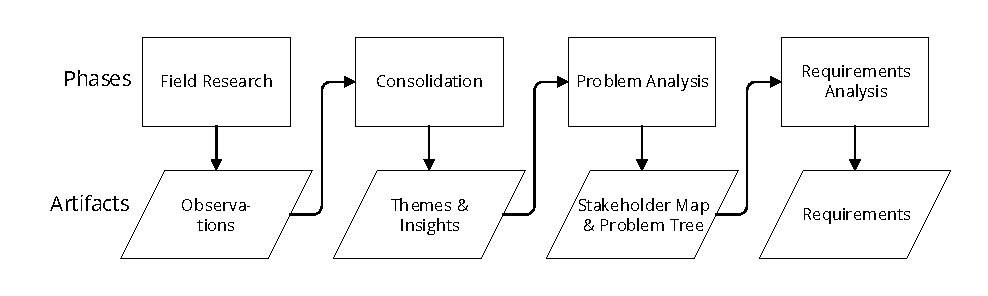
\includegraphics[width=0.99\textwidth]{../figures/20180115-DRF-Research-Process-Flow.pdf}
\caption{Research Process for Requirements Analysis}\label{fig:research-process}
}
\end{figure}

\textbf{Field research} was conducted at the headquarters of the \gls{sme}-sized \gls{isv} medatixx (cf.~\cref{sec:company-characteristics}) to elicit observations as basis for systematic problem analysis.
Methods from \gls{hcd}'s Inspire phase were employed: \emph{Recruiting Tools} helped identify relevant stakeholders for interviewing, including senior management (``Leiter Softwareproduktion'' -- Head of Development), middle management (``Abteilungsleiter Softwareproduktion'' -- Head of Software Development Department) and staff (software engineers, software testers, scrum masters, product owners, DevOps, maintenance) and, following the \emph{Extremes and Mainstream} method including both proponents and opponents of \gls{Web Migration}.
A \emph{Guided Tour} was taken to get to know the different development teams, organizational structures, and work environment.
The observations were elicited using individual and group \emph{Interviews} and using in-context \emph{Immersion}.
This method was particularly fruitful, comprising a one-week integration in a scrum team, actively participating in development activities and meetings.
This provided a good understanding of the daily development practice, expertise level of staff and a solid trust basis for interviews and subsequent feedback cycles, in particular for the development of the Annotation Platform presented in \cref{sec:platform}.
More than 50 observations of the field research phase were captured and organized using Trello\footnote{\url{https://trello.com/} Retrieved: 6.12.2019} cards. %\pagebreak

\textbf{Consolidation} was used to abstract from the concrete observations into themes that capture relevant and recurring problem patterns.
This was supported by \gls{hcd}'s Ideation phase methods.
\emph{Find Themes} in combination with the collaborative filtering proposed in the \emph{Top Five} method was used to cluster the observations and identify the most relevant problem areas, e.g. migration effort, available staff expertise, and unknown potentials of a \gls{web}-based solution.
\emph{Insight statements} were created for the themes from observations.
The themes and insights were captured on post-its to provide the input for problem analysis.

\textbf{Problem Analysis} considered the relationships between the insights and themes to create a systematic view of the problem domain.
According to \gls{hcd}'s \emph{Create Frameworks} method, an initial relational map was created.
\gls{lfa} \emph{stakeholder analysis} was conducted to capture the stakeholder map, which systematically describes characteristics and intentions of the involved roles.
The problem hierarchy was identified bottom-up from the insights, and themes and their cause-effect relationships were represented as an \gls{lfa} \emph{problem tree}, identifying three major sub-trees of overloading, doubts about feasibility and doubts about desirability.
The results of the problem analysis phase were iteratively improved through a feedback loop with the \gls{isv} and are outlined in the next subsection.

\hypertarget{tbl:research-methods}{}
\begin{longtable}{@{}ll@{}}
\caption{\label{tbl:research-methods}Methods used in Research phases}\tabularnewline
\toprule
\begin{minipage}[b]{0.28\columnwidth}\raggedright
Phase\strut
\end{minipage} & \begin{minipage}[b]{0.66\columnwidth}\raggedright
Methods\strut
\end{minipage}\tabularnewline
\midrule
\endfirsthead
\toprule
\begin{minipage}[b]{0.28\columnwidth}\raggedright
Phase\strut
\end{minipage} & \begin{minipage}[b]{0.66\columnwidth}\raggedright
Methods\strut
\end{minipage}\tabularnewline
\midrule
\endhead
\begin{minipage}[t]{0.28\columnwidth}\raggedright
Field Research\strut
\end{minipage} & \begin{minipage}[t]{0.66\columnwidth}\raggedright
\gls{hcd} Recruiting Tools, Interviews, Extremes and Mainstream, Immersion, Guided Tour\strut
\end{minipage}\tabularnewline
\begin{minipage}[t]{0.28\columnwidth}\raggedright
Consolidation\strut
\end{minipage} & \begin{minipage}[t]{0.66\columnwidth}\raggedright
\gls{hcd} Top Five, Find Themes, Create insight statements\strut
\end{minipage}\tabularnewline
\begin{minipage}[t]{0.28\columnwidth}\raggedright
Problem Analysis\strut
\end{minipage} & \begin{minipage}[t]{0.66\columnwidth}\raggedright
\gls{hcd} Create Frameworks, LFA Stakeholder Analysis, LFA Problem Tree\strut
\end{minipage}\tabularnewline
\bottomrule
\end{longtable}

\hypertarget{sec:problem-analysis-results}{%
\subsection{Results}\label{sec:problem-analysis-results}}
\vspace{10pt}

Problem analysis phase comprises two parts: stakeholder analysis and problem tree analysis.
For stakeholder analysis, we identified stakeholders and their characteristics in terms of their interests and how they are affected by a \gls{Web Migration}, their capacity and motivation, and possibilities to address and engage them.
For problem tree analysis, we identified stakeholder problems and their relationships.
The stakeholder and problem tree analysis results were presented and validated with the scenario stakeholder, and feedback was incorporated in several feedback cycles.

\textbf{Stakeholder Analysis}.
\Cref{tbl:stakeholders} shows the results of stakeholder analysis.
It comprises three groups of stakeholders: \gls{isv} stakeholders, customer stakeholders, and external stakeholders.
The \gls{isv} stakeholders are divided into two distinct roles: \emph{Management} and \emph{Software Engineers}.
Management is responsible for the decision to migrate and is aware of the risks and thus must be addressed through \gls{risk management} and communication of benefits.
Software Engineers are the group of potential actors of \gls{Web Migration}; they define the requirements for migration activities through their expertise and development processes, and tailored methods need to be provided that reduce migration workload.
We use the term \gls{migrationengineer} to refer to a Software Engineer who is performing \gls{Web Migration} activities.
Migration Engineers are to be considered a sub-class of Software Engineers, i.e.~all super-class characteristics apply.
Two customer stakeholders exist: the \emph{doctor's offices} are the direct customer of the \gls{pms} \gls{isv} whereas \emph{patients} are the customers of the customers and benefit the most from innovative features and improved usability and interactivity.
Furthermore, \emph{competitors} are external stakeholders affected by the effects on the market share of increased competitiveness of the \gls{isv} through \gls{Web Migration} and \emph{companies with similar situation}, i.e.~other \glspl{isv} with non-\glslink{web}{Web}\glspl{Legacy System} and large user bases can benefit from the dissemination of results to apply to their situation.

\textbf{Problem Tree Analysis}.
The knowledge about the stakeholders together with themes and insights from the consolidation phase feeds into the analysis of problems and problem relationships.
The problem hierarchy is presented in \cref{fig:problem-tree}.
While it was created bottom-up, starting with insights, we briefly outline the problem tree top-down for easier understanding.
The arrows in the \gls{lfa} tree indicate cause-effect relationships, with effects represented in the direction of the arrows and causes in the opposite direction.
The root-level problem is the competitiveness of the \gls{isv} company. The effects of this problem, such as losing market shares to the competition, are not shown for brevity.
This competitiveness is jeopardized by both the consequences of maintaining a \gls{Legacy System} and \gls{Technical Debt} (cf.~\cref{sec:situation}) leading to \emph{overloading} of staff and the \emph{hesitation to commence \gls{Web Migration}} due to \emph{doubts about feasibility and desirability} \autocite[cf.~also to resistance from organization in][]{Khadka2014ProfessionalsModernization,Sneed2010ReMiP}.
The \glslink{Legacy System}{legacy}-characteristic causes of overloading, such as low maintainability due to \emph{side-effects}, \emph{technological deprecation}, \emph{multi-platform environment}, and \emph{limited time \& resources}, are pushing factors in favor of a \gls{Web Migration}.
On the other hand, risk and effort of a \gls{Web Migration} constitute \emph{doubts about feasibility and desirability}.
In particular, \emph{limited time and resources} for conducting the migration, \emph{unknown plausibility of a \glslink{web}{Web}-based version}, difficult \emph{integration into ongoing development}, and a \emph{lack of knowledge of methods and technologies} regarding migration and staff with \emph{\gls{Web Engineering} expertise} feed into feasibility doubts.
Likewise, \emph{lack of a deeper understanding of potential benefits}, the \emph{risk of losing poorly documented knowledge}, and \emph{potential impact on existing customers} through abrupt changes form doubts about the desirability of \gls{Web Migration}.
The root causes on the lowest level of the problem tree are \emph{architectural degradation} of the \glspl{Legacy System}, \emph{missing documentation and experience of \glslink{Legacy System}{legacy} code}, a \emph{strict release cycle regime} due to regulatory and contractual constraints, lack of \emph{staff with \gls{Web Engineering} expertise} and a large existing \emph{customer base whose workflows are oriented on the user interaction of the software products}.
These situational problems impose constraints on potential solutions and are represented as stakeholder requirements in the next section.
%The latter three problems are situational problems that impose constraints on potential solutions as represented in requirements \cref{c:4} Agile, \cref{c:3} Exp and \cref{c:2} Reuse.

\vspace{-25pt}
\hypertarget{sec:requirements}{%
\section{Requirements}\label{sec:requirements}}
\vspace{7pt}

In this section, requirements for assessing the state of the art are elicited based on the motivation and problem outlined in the introduction and the scenario-based problem analysis above.
These requirements are divided into two groups:

\begin{itemize}
\tightlist
\item
  \textbf{Scope requirements} are detailing criteria that ensure that a solution addresses the scope set by the main research question \cref{rq:1}.
\item
  \textbf{Stakeholder requirements} are detailing criteria that ensure the appropriateness of a solution for an \gls{isv} as detailed in the scenario based on the problem analysis results in \cref{sec:problem-analysis-results}, representing a more detailed view on effort and risk from research questions \cref{rq:2} and \cref{rq:3}.
\end{itemize}

\Cref{tbl:requirements} provides an overview of all scope and stakeholder requirements, introduces short IDs for use in the following text, shows their relation to the research questions, and indicates their significance according to RFC 2119 levels MUST\footnote{for absolute requirements fulfillment of which is mandatory} and SHOULD\footnote{for requirements fulfillment of which is recommended} \autocite{IETF2119MustShould}. Their relationships with the research questions are shown in \cref{fig:rq-req}.

In the following, each requirement is detailed, and a mapping onto a three-level assessment scheme (not satisfied, partially satisfied, satisfied) is presented. The mapping is defined based on satisfaction criteria per requirement.

\begin{longtable}[]{@{}lll@{}}
\caption{\label{tbl:requirements}Scope and Stakeholder Requirements}\tabularnewline
\toprule
ID & Requirement & Level\tabularnewline
\midrule
\endhead
\multicolumn{3}{@{}l}{\textbf{Scope Requirements}}\tabularnewline
\cref{s:1} Initial & Initial Phase Support &  MUST\tabularnewline
\cref{s:2} Web & Web Application Target &  MUST\tabularnewline
\multicolumn{3}{@{}l}{\textbf{Stakeholder Requirements}}\tabularnewline
\cref{c:1} Risk & Risk Management &  SHOULD\tabularnewline
\cref{c:2} Reuse & Reuse of Legacy Assets &  SHOULD\tabularnewline
\cref{c:3} Exp & Expertise \& Tool Support &  SHOULD\tabularnewline
\cref{c:4} Agile & Agile Development Process Integration &  SHOULD\tabularnewline
\bottomrule
\end{longtable}

\pagebreak

\begin{figure}[hbt]
\hypertarget{fig:rq-req}{%
\centering%
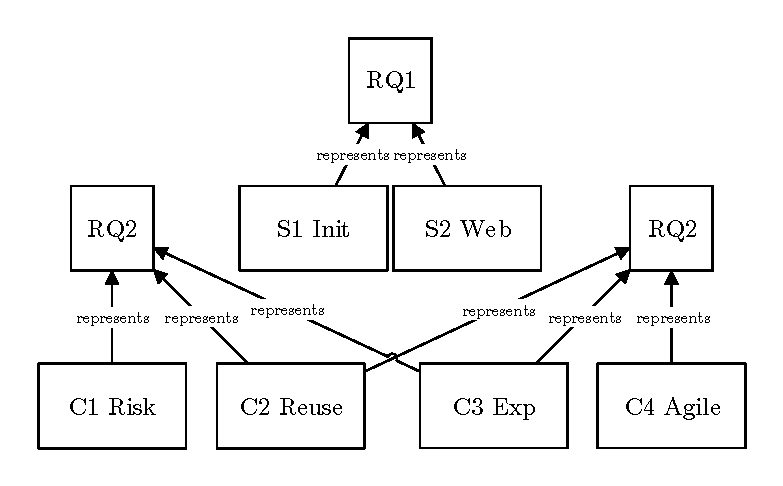
\includegraphics[width=0.75\textwidth]{../figures/rq-req.pdf}%
\caption[Research Questions and Requirements]{Concept Map of Relationships between Research Questions and Requirements}%
\label{fig:rq-req}%
}
\end{figure}

\hypertarget{scope-requirements}{%
\subsection{Scope Requirements}\label{scope-requirements}}
\vspace{10pt}

The following two requirements detail the scope of this thesis to consider \gls{Web Migration} approaches that support the initial phase of a \gls{Web Migration} and which are designed to produce \glspl{Web Application} from \glspl{Legacy System} as of \cref{rq:1}.

\begin{thesisscoperequirement}{Initial Phase Support}{s:1}
\glspl{isv} find it particularly difficult to commence a \gls{Web Migration} \autocite{Heil2017Survey,Heil2018ReWaMP}.
This requirement, therefore, assesses approaches with regard to how much they support an \gls{isv} to overcome the initial resistance.
According to the \gls{remip} \autocite{Sneed2010ReMiP}, any software migration process can be divided into four phases: Preliminary Study, Conceptualization and Design, Migration and Transition, and Closing down.
A similar phase distinction is also found in EU FP7 REMICS \autocite{Krasteva2013REMICSAgile}: requirements and feasibility, recover, migrate, validation.
The first two phases in both reference models comprise the initial activities before the actual \gls{Transformation} is started in the third phase, with activities including evaluation of the \gls{Legacy System}, legacy analysis, and definition of migration strategy and \gls{target system}.
Technically required for any \gls{Reengineering} or \gls{Transformation} approach, recovery of knowledge plays a special role in migration and is therefore considered separately in \emph{\cref{c:2} Reuse}.
Thus, approaches covering activities from the first two phases that are not related to recovery are considered to support the initial phase to some extent.
However, the mainly technical perspective of the reference models' phases ignores the importance of communication of the necessity and benefits of \glslink{Software Modernization}{modernization} -- communicating the business value is crucial for creating a \gls{business case}\footnote{``a documented economic feasibility study used to establish validity of the benefits of a selected component lacking sufficient definition and that is used as a basis for the authorization of further project management activities'' \autocite{ISO/IEEE24765Vocabulary}} for migration \autocite{AmazonWebServices2018Migration,Khadka2016PHD,Menychtas2014ARTISTJournal,Batlajery2014IndustrialSurveyModernization,Khadka2014ProfessionalsModernization} that justifies the project cost with benefits \autocite{Sneed1995CostBenefit} -- to address migration resistance within organizations \autocite{Khadka2014ProfessionalsModernization,Sneed2010ReMiP}.
A suitable approach should, therefore, additionally provide appropriate methods and tools to supply \glspl{artifact} that can be used as a basis for communicating the necessity and benefits of migration and supporting the decision making.

The satisfaction criterion of initial phase support is the support for both the technical and the communication perspective of the initial phase, which means that activities prior to the actual migration are addressed and include support for communicating necessity and benefits.
The requirement is partially satisfied if activities prior to actual migration are addressed, but communication is ignored.
Finally, the requirement is considered not satisfied if only activities from the third and fourth \gls{remip}/REMICS phase are addressed.
\end{thesisscoperequirement}

%(Target Environment)
\begin{thesisscoperequirement}{Web Application Target}{s:2}
Due to the advantages of the \gls{web} platform \autocite{Gitzel2007WebEngineeringMDD,Knorr2003WebAsPlatform} and to meet \glspl{isv}' migration objectives with regard to the integration of roles and interactivity as described in \cref{sec:situation}, a \glslink{web}{Web}-based system is required.
\gls{Software Migration} is the process of moving an existing software system from one environment to another \autocite{SWEBOK2014}.
Generic software migration approaches, however, do not sufficiently address the \gls{web} paradigms, like the asynchronous request-response communication model, client-server separation in the spatial and technological dimension, or URL-based resources and addressable \gls{ui} states/navigation patterns \autocite{Heil2017Survey}.
In the context of \gls{Web Migration}, the \gls{target environment} is the \gls{web} platform.
\gls{Web Migration} approaches comprise different types of target \glspl{Web System} (cf.~\cref{def:websystem}) such as \glspl{Web Application}, \gls{soa}-based, and Cloud-based systems \autocite{Heil2017Survey}.
Only a subset of these approaches explicitly focuses on \glspl{Web Application} as defined in \cref{def:webapplication}.
Since the migration objectives require a \gls{Web Application}, including a \glslink{web}{Web}-based user interface, approaches for \gls{soa} or Cloud migration are only partially applicable.
It is important to note that, according to \cref{def:webapplication}, not every \gls{Web System} with a \glslink{web}{Web}-based \gls{ui} is a \gls{Web Application} since in addition, provision of \glslink{web}{Web}-specific resources is required.

The satisfaction criterion of the Web Application Target requirement is the \gls{Web Application} nature of the software that is produced by an approach, which means that the resulting software system is based on \gls{web} technologies and standards and provides Web-specific resources through a \glslink{web}{Web}-based user interface.
The requirement is partially satisfied if the software is a \gls{Web System}, but lacks the aspect of a \glslink{web}{Web}-based user interface.
Finally, the requirement is considered not satisfied if an approach only addresses the development or migration of software in general without consideration of the \gls{web} as target environment.
\end{thesisscoperequirement}

\pagebreak
\hypertarget{stakeholder-requirements}{%
\subsection{Stakeholder Requirements}\label{stakeholder-requirements}}
\vspace{10pt}

The following four requirements detail concerns about commencing a \gls{Web Migration} from an \gls{isv}'s perspective by further detailing risk and effort from \cref{rq:2,rq:3}.


\begin{thesisstakeholderrequirement}{Risk Management}{c:1}
As outlined \cref{sec:problem}, any \gls{Software Modernization} involves a high risk, which makes \glspl{isv} hesitant to commence this process \autocite{Khadka2014ProfessionalsModernization,Canfora2000Decomposing,Bisbal1999LegacyInformationSystems,Heil2018ReWaMP}.
The risks can be divided into two categories: \emph{risks of migration process failure} and \emph{risks of failure of the resulting new system}.
Both categories require appropriate strategies to manage and decrease the risk level.
Redevelopment approaches from scratch without consideration of the existing software system and \glspl{artifact}, called ``Cold Turkey'' \autocite{Brodie1995Migrating} and holistic cutover strategies, called ``Big Bang'' \autocite{Bisbal1999LegacyInformationSystems}, have a high risk of failure \autocite{Sneed2010SoftwareMigration,Bisbal1999LegacyInformationSystems}.
Typical \gls{risk management} \autocite{ISO/IEEE24765Vocabulary} and mitigation strategies for large migration projects are to follow an incremental migration process \autocite{Colosimo2007ControlledExperiments,Sneed2010SoftwareMigration} -- originally introduced as package-oriented incremental ``\emph{chicken little}'' strategy \autocite{Brodie1995Migrating} -- and to use pilot projects as trial migrations to identify obstacles such as feasibility threats early on \autocite{AmazonWebServices2018Migration,Sneed2010SoftwareMigration}.
\emph{Feasibility studies} assessing the technical feasibility and economic viability \autocite{ISO/IEEE24765Vocabulary} are another means of basic \gls{risk management} commonly observed.
\emph{Portfolio analysis} is a \gls{risk management} method to identify potential migration candidates using a quadrant graph of business value and technical quality \autocite{Seacord2003ModernizingLS,Sneed1995CostBenefit}.
For these candidates, stakeholders and requirements are identified to finally make the \gls{business case}, a document to support decision making and planning \autocite{AmazonWebServices2018Migration,Seacord2003ModernizingLS}.
Advanced \gls{risk management} methods should thus contribute to the \gls{business case} \autocite{Seacord2003ModernizingLS} in order to address the desirability doubts in \cref{sec:problem-analysis-results}.
\glslink{Software Modernization}{Modernization} bears the risk of losing valuable tacit knowledge about business processes, rules, etc.
\autocite{Aversano2001,Distante2006a,Sneed2010SoftwareMigration,Wagner2014} which are not explicitly documented but only implicitly represented by the \glslink{Legacy System}{legacy} source code \autocite{Khadka2014ProfessionalsModernization,Heil2017Survey}. 
This knowledge represents high financial value, resulting from high investments in the past \autocite{Lucia2009METAMORPHOS}.
As shown in \cref{sec:problem-analysis-results}, the risk of losing knowledge is a problem for \glspl{isv}.
A \emph{risk-managed \glslink{Software Modernization}{modernization}} strategy \autocite{Seacord2003ModernizingLS} therefore, should provide methods to re-discover, sustain, and manage this knowledge to make it useable for subsequent \glslink{Software Modernization}{modernization} activities.

The satisfaction criterion of the Risk Management requirement is the \gls{risk management} of the \gls{Web Migration}, which means that at least one basic \gls{risk management} practice beyond an incremental process is combined with advanced strategies contributing to the \gls{business case} and the securing of existing knowledge against loss during migration.
The requirement is partially satisfied if the approach only employs basic \gls{risk management} practices beyond an incremental process model, but lacks contribution to the \gls{business case} and the securing of knowledge.
Finally, the requirement is considered not satisfied if an approach does not take into account \gls{risk management}.
\end{thesisstakeholderrequirement}

\begin{thesisstakeholderrequirement}{Reuse of Legacy Assets}{c:2}
%TODO:RENAME\_continuity\_of\_functionality\_and\_UIX?
Redevelopment from scratch -- sometimes also referred to under the category of \emph{replacement} \autocite{Almonaies2010SOAStrategies} -- is a major strategy for \gls{Legacy Modernization} \autocite{Wagner2014,Khadka2016PHD,Sneed2010SoftwareMigration,Almonaies2010SOAStrategies,Bisbal1999LegacyInformationSystems}.
However, its lack or limited reuse of existing \glslink{Legacy System}{legacy} assets incurs significant development cost \autocite{Khadka2016PHD} and bears the risk of the new system not being as functional as the old one \autocite{Almonaies2010SOAStrategies}.
Maintaining a system's functionality throughout any \gls{Software Modernization} means to maintain the domain knowledge and business logic \autocite{Wagner2014}.
From an end user's perspective, it also means continuity in the user interface and user interaction.
As seen in \cref{sec:problem-analysis-results}, companies aim at maintaining the look and feel of the \glslink{Legacy System}{legacy} user interface to avoid forcing end users to change their working habits \autocite{Rodriguez-Echeverria2012MIGRARIA,Lucia2008,Distante2002}.
Existing \emph{legacy artifacts}\footnote{In this thesis we distinguish between \glspl{artifact} and \glspl{asset}.
``A software artifact is a tangible machine-readable document created during software development.
Examples are requirement specification documents, design documents, source code, and executables.'' \autocite{OMG2016KDM}, \autocite[cf.~\emph{physical asset}][]{ISO/IEEE24765Vocabulary}} of an \gls{isv} comprise the \glslink{Legacy System}{legacy} source code and the running \gls{Legacy System} itself, whereas \emph{assets}\footnote{An asset is an ``item, thing or entity that has potential or actual value to an organization'' \autocite{ISO/IEEE24765Vocabulary}.
``A software asset is a description of a partial solution \ldots{} or knowledge \ldots{} that engineers use to build or modify software products.'' \autocite{OMG2016KDM} Parts of software can be an artifact and an asset at the same time (e.g.~documentation).
Unless explicitly codified, we consider requirements, models, rules, etc.
represented by the legacy source code as assets but not artifacts, since they are not tangible \autocite[cf.~\emph{intangible assets}][]{ISO/IEEE24765Vocabulary}.} like documentation, requirements, or models originally used for production are typically missing.
\autocite{Wagner2014,Bisbal1999LegacyInformationSystems,Sneed2010SoftwareMigration,warren2012renaissance,Batlajery2014IndustrialSurveyModernization,Lucia2008}.
Thus, original requirements and models need to be rediscovered from existing software \glspl{artifact} to enable reuse, employing appropriate \gls{Reverse Engineering} techniques such as static analysis of \glslink{Legacy System}{legacy} source code or dynamic analysis of system behavior \autocite{Lucia2008}.
A suitable approach must promote rediscovery, management, and reuse of assets in existing software \glspl{artifact} to increase the continuity of functionality \autocite{Almonaies2010SOAStrategies} and user interaction between \glslink{Legacy System}{legacy} and new system in order to reduce the development cost \autocite{Khadka2016PHD} and accelerate \glslink{Software Modernization}{modernization} compared to redevelopment from scratch \autocite{Sneed2010SoftwareMigration}.

The satisfaction criterion of the Reuse of Legacy Assets requirement is the degree of reuse of assets from existing software \glspl{artifact}, which means that \glslink{Legacy System}{legacy} source code and the running \gls{Legacy System} itself should be used as the source for maintaining functionality and user interaction across \glslink{Legacy System}{legacy} and new system.
The requirement is partially satisfied if either only functionality or only user interaction is maintained.
Finally, the requirement is considered not satisfied if existing assets are not taken into account for the continuity of functionality or user interaction.
\end{thesisstakeholderrequirement}

\begin{thesisstakeholderrequirement}{Expertise \& Tool Support}{c:3}
\emph{Expertise} of the available staff is a crucial resource for any \gls{Software Modernization} \autocite{Khadka2014ProfessionalsModernization,Batlajery2014IndustrialSurveyModernization,Sneed2010SoftwareMigration,Seacord2003ModernizingLS}.
While expertise in the source technology base in \glspl{isv} with continuous maintenance and development activities due to existing contracts and strict release cycles as described in \cref{sec:company-characteristics} is typically high, experience with older parts of the \gls{Legacy System} can be significantly lower due to retirement or change of job of the original developers \autocite{Khadka2016PHD,Batlajery2014IndustrialSurveyModernization,Khadka2014ProfessionalsModernization}, called \emph{erosion of soft knowledge} \autocite{Khadka2014ProfessionalsModernization}.
Lack of staff experienced in \gls{Software Modernization} itself is a feasibility threat \autocite{Sneed2010SoftwareMigration,Seacord2003ModernizingLS}.
For \gls{Web Migration}, additional \gls{Web Engineering} expertise is required due to the specifics of the target environment (cf.~\emph{\cref{s:2} Web}), but typically not existing in \glspl{isv} of traditional non-\glslink{web}{Web} \glspl{Desktop Application} \autocite{Fowley2017CloudSME}, as shown in \cref{sec:problem-analysis-results}.
For an \gls{isv} to be able to commence a \gls{Web Migration} with existing staff and expertise, approaches need to consider the four experience levels explained above in terms of its requirements and provide supporting infrastructure for partial or full \emph{automation} and proper \emph{guidance} in the migration process.
The effort for \gls{Reverse Engineering} and migration activities can be significantly reduced by suitable support tools \autocite{Lucia2009METAMORPHOS}, which only see limited use in the industry \autocite{Torchiano2008ItalianSurvey}.
Additional staff or outsourcing\footnote{cf.~also to \autocite{Razavian2012} for strategy differences between in-house and outsourced migration projects} the entire migration is not desirable due to limited financial resources and complexity of the \gls{Legacy System}, respectively (cf.~\cref{sec:company-characteristics}).

The satisfaction criterion of the Expertise \& Tool Support requirement is the expertise requirements, which means that suitable approaches are feasible with existing staff based on experience levels in \glslink{Legacy System}{legacy} technology, \gls{Legacy System}, target technology, and migration, supported, if necessary, through appropriate tools and proper guidance in the migration process.
The requirement is partially satisfied if the approach only meets the staff expertise, but lacks tool support.
Finally, the requirement is considered not satisfied if additional staff or outsourcing is required.
\end{thesisstakeholderrequirement}

\begin{thesisstakeholderrequirement}{Agile Development Process Integration}{c:4}
Software providers have \emph{ongoing development and maintenance activities}, as described in \cref{sec:problem-analysis-results}.
Organization structures are representing these activities with teams' responsibilities assigned to maintenance of products or components and implementation of new features, following \emph{agile development methodologies} that govern work organization in terms of process, roles and artifacts \autocite{Beedle2002Scrum}.
The importance of supporting existing ways of working has only recently been acknowledged in lean perspectives on migration research \autocite{Razavian2014a}.
Additional activities required by \gls{Web Migration} thus need to be integrated with day-to-day development activities of existing teams to avoid re-structuring or even exclusively dedicating teams to migration \autocites[cf.~\emph{modernization teams} in][]{Krasteva2013REMICSAgile}[\emph{migration factory teams} in][]{AmazonWebServices2018Migration}.
Of the seven disciplines according to \gls{remip} \autocite{Sneed2010ReMiP,Gipp2007ReMiP}, target design, implementation, test, and deployment are very similar to traditional forward software engineering and therefore easier to integrate.
In contrast, requirements analysis -- for migration, this means eliciting un-documented requirements from \glslink{Legacy System}{legacy} \glspl{artifact}, mainly the legacy code -- legacy analysis, and strategy selection are migration specific activities that are significantly different from regular software engineering activities and therefore more difficult to integrate.
Integration is not only required at the process level in terms of activities, but also for \glspl{artifact} that are created and drive the development.

The satisfaction criterion of the Agile Development Process Integration requirement is the completeness of development integration, which means that all migration activities are integrated into ongoing development processes, and integration is also achieved at the \glspl{artifact} level.
The requirement is partially satisfied if not all activities are integrated, or integration of \glspl{artifact} is lacking.
Finally, the requirement is considered not satisfied if an approach does not integrate with ongoing development and is designed to be stand-alone.
\end{thesisstakeholderrequirement}

\vspace{-15pt}
\hypertarget{sec:requirements.summary}{%
\section{Summary}\label{sec:requirements.summary}}
\vspace{15pt}

This chapter introduced a guiding scenario of an \gls{sme}-sized \gls{isv} struggling to bring its non-\glslink{web}{Web} \glspl{Legacy System} to the \gls{web} and detailed the characteristics of the company, software development, and \gls{Legacy System}, and described migration objectives.
The problem analysis has detailed the effort and risk factors and introduced a model of stakeholder roles for devising a suitable solution.
Based on the problem analysis results, six requirements were elicited. 
The two scope requirements represent the problem identified as the scope of this thesis in \cref{rq:1}, i.e., support for the initial phases of \gls{Web Migration} and \glspl{Web Application} as target architecture.
The four stakeholder requirements addressing \cref{rq:2,rq:3} are derived from the problems of the scenario stakeholder regarding the management of risk, reuse of \glslink{Legacy System}{legacy} assets to ensure continuity of functionality and user interaction, suitability for available expertise and tool support, and integration into ongoing agile development and maintenance activities.
For each of the requirements, a three-level assessment scheme was introduced, enabling the evaluation of existing \gls{Web Migration} approaches regarding their suitability in the following chapter.
